%\documentclass{beamer} %voce pode usar este modelo tambem
\documentclass[t,handout,9pt]{beamer}
\usepackage{graphicx}
\usepackage{url}
\usepackage[british]{babel}
\batchmode
% \pgfpagesuselayout{4 on 1}[letterpaper,landscape,border shrink=5mm]
\usepackage{amsmath}
\usepackage{amssymb}
\usepackage{amsfonts}
\usepackage{enumerate}
\usepackage{epsfig}
\usepackage{bbm}
\usepackage{calc}
\usepackage{adjustbox}
\usepackage{color}
\usepackage{ifthen}
\usepackage{capt-of}
\usepackage{float}
\usepackage{booktabs}
\usepackage{dcolumn}
\usepackage{multicol}
\usepackage{hyperref}
\usepackage[flushleft]{threeparttable}
\usepackage{subcaption}
\usepackage{adjustbox}
\usepackage{ragged2e}
\usepackage{xcolor}
\usepackage{pgfpages}
%\usepackage{showframe}

\usepackage{cmbright}

\renewcommand\ttdefault{cmvtt} % selects CM typewriter

\usepackage[utf8]{inputenc} % Required for inputting international characters
\usepackage[T1]{fontenc} 	% Output font encoding for international characters

%\DeclareFontShape{OT1}{cmss}{b}{n}{<->ssub * cmss/bx/n}{}

\usetheme[compress]{Berlin}
\definecolor{sapienza}{RGB}{0, 49, 83}
\usecolortheme[named=sapienza]{structure}

\usepackage[backend=bibtex,style=alphabetic,giveninits=true,url=false,eprint=false,doi=false]{biblatex}
\DeclareNameAlias{sortname}{last-first}
\renewcommand*{\nameyeardelim}{\addcomma\addspace}
\renewcommand*{\bibfont}{\footnotesize}
\addbibresource{example.bib}
\setbeamerfont{footnote}{size=\tiny}

\setbeamerfont{title}{size=\LARGE}

% reduce spaces between tables/figures and caption
\usepackage[font=small,skip=1pt]{caption}

%% pgf plots stuff
%\usepackage{pgfplots}
%\pgfplotsset{compat=newest}
%% the following commands are needed for some matlab2tikz features
%\usetikzlibrary{plotmarks}
%\usetikzlibrary{arrows.meta}
%\usepgfplotslibrary{patchplots}

% one navigation dot per slide trick
\AtBeginSection[]{\subsection{}}

% fix misbehave for allowframebreaks
\usepackage{etoolbox}
\makeatletter
\patchcmd{\slideentry}{\ifnum#2>0}{\ifnum2>0}{}% replace the subsection number test with a test that always returns true
% use frame numbers instead of subsection slide numbers so that frames broken over slides get separate circles
\patchcmd{\slideentry}{\c@subsectionslide}{\c@framenumber}{}{\@error{unable to patch}}
\patchcmd{\beamer@writeslidentry}{\c@subsectionslide}{\c@framenumber}{}{\@error{unable to patch}}

% date in footer trick
\makeatletter
  \setbeamertemplate{footline}{%
    \begin{beamercolorbox}[colsep=1.5pt]{upper separation line foot}
    \end{beamercolorbox}
    \begin{beamercolorbox}[ht=2.5ex,dp=1.125ex,%
      leftskip=.3cm,rightskip=.3cm plus1fil]{author in head/foot}%
      \leavevmode{\usebeamerfont{author in head/foot}\insertshortauthor}%
      \hfill%
      {\usebeamerfont{institute in head/foot}\usebeamercolor[fg]{institute in head/foot}\insertshortinstitute}%
    \end{beamercolorbox}%
    \begin{beamercolorbox}[ht=2.5ex,dp=1.125ex,%
      leftskip=.3cm,rightskip=.3cm plus1fil]{title in head/foot}%
      {\usebeamerfont{title in head/foot}\insertshorttitle\hfill\insertshortdate}%
    \end{beamercolorbox}%
    \begin{beamercolorbox}[colsep=1.5pt]{lower separation line foot}
    \end{beamercolorbox}
  }
\makeatletter

% remove dot for titlepage and Outline
\makeatletter
\let\old@beamer@writeslidentry\beamer@writeslidentry
\def\beamer@writeslidentry{%
  \expandafter\beamer@ifempty\expandafter{\beamer@framestartpage}{}% does not happen normally
  {%else
    \clearpage\beamer@notesactions%
  }
}
\makeatother

% let's number figure captions
\setbeamertemplate{caption}[numbered]

% trick for grouping equations
\newenvironment{rcases}
  {\left.\begin{aligned}}
  {\end{aligned}\right\rbrace}

%-------------------------Titulo/Autores/Orientador------------------------------------------------
\title[Introduction to Computer Programming]{Introduction to Computer Programming}
\date[A.Y. 2024-2025]{\\A.Y. 2024-2025}
\author[Alessio Martino]{Prof. Alessio Martino\\
\smallskip
{\small \href{mailto:amartino@luiss.it}{\texttt{amartino@luiss.it}}}\\
\smallskip
}
\institute[15/10/2024]{Department of Business and Management\\Viale Romania 32, 00197 Rome\\[\bigskipamount]

\includegraphics[scale=0.4]{Figures/cliente-luiss.png}%
}

%-------------------------Logo na parte de baixo do slide------------------------------------------
%\pgfdeclareimage[height=0.7cm]{senac-logo}{senac-logo.pdf}
%\logo{\pgfuseimage{senac-logo}\hspace*{0.5cm}}

%-------------------------Este código faz o menuzinho bacana na parte superior do slide------------
%\AtBeginSection[]
%{
%  \begin{frame}<beamer>
%    \frametitle{Outline}
%    \tableofcontents[currentsection]
%  \end{frame}
%}
%\beamerdefaultoverlayspecification{<+->}
% -----------------------------------------------------------------------------

\begin{document}
% -----------------------------------------------------------------------------

%---Gerador de Sumário---------------------------------------------------------

\frame[noframenumbering]{
	\titlepage
}

% begin personalization stuff
\setbeamertemplate{navigation symbols}{%
	\insertslidenavigationsymbol
	\insertframenavigationsymbol
	\insertsubsectionnavigationsymbol
	\insertsectionnavigationsymbol
	\insertdocnavigationsymbol
	\insertbackfindforwardnavigationsymbol
	\hspace{1em}%
	\usebeamerfont{footline}
	\insertframenumber/\inserttotalframenumber%
}
\setbeamertemplate{itemize items}[circle]
\setbeamertemplate{enumerate items}[circle]
\setbeamertemplate{bibliography item}{\insertbiblabel}
% end personalization stuff

\section[]{}
\begin{frame}{Outline}
	\tableofcontents
\end{frame}
%\begin{frame}{Outline}
%\begin{multicols}{2}
%  \tableofcontents
%\end{multicols}
%\end{frame}
%---Fim do Sumário------------------------------------------------------------

% reset navigation dots for other slides
\makeatletter
\let\beamer@writeslidentry\old@beamer@writeslidentry
\makeatother

% -----------------------------------------------------------------------------
\section{Introduction}
\begin{frame}{Introduction}
\vfill
In Python, lists
\begin{itemize}
	\item are ordered \textcolor{red}{sequences} of items that can be accessed via index\footnote{Remember: Python is 0-based!}
	\item are denoted by \textcolor{red}{square brackets}, i.e. \texttt{[ ]}
\end{itemize}
\vfill
A list contains \textcolor{red}{elements}, that can either be:
\begin{itemize}
	\item homogeneous (e.g., all integers, all strings, ...)
	\item heterogeneous (less common)
\end{itemize}
\vfill
Conversely to strings, lists are \textcolor{red}{mutable}:
\begin{itemize}
	\item elements can be changed
\end{itemize}
\vfill
\end{frame}
%
\subsection{Indices and Ordering}
\begin{frame}
\vfill
\begin{table}[]
\begin{flushleft}
\begin{tabular}{ll}
\texttt{a\_list = [ ]} & \# an empty list\\
\texttt{L = [2, 'a', 4, [1,2]]} & \# an heterogeneous list \\
& \\
\texttt{len(L)} &  \# evaluates to \texttt{4}\\
\texttt{L[0]} &  \# evaluates to \texttt{2}\\
\texttt{L[2] + 1} &  \# evaluates to \texttt{5}\\
\texttt{L[3]} &  \# evaluates to \texttt{[1,2]} ... another list\\
\texttt{L[4]} &  \# throws an error\\
& \\
\texttt{i = 2} &  \\
\texttt{L[i-1]} &  \# evaluates to \texttt{'a'}\\
& \\
\texttt{L[1:3]} &  \# evaluates to \texttt{['a', 4]}\\
\end{tabular}
\end{flushleft}
\end{table}
\vfill
\end{frame}
%
\section{Mutability}
\begin{frame}{Mutability}
\vfill
\begin{block}{Recall}
Lists are \textcolor{red}{mutable}.
\end{block}
The assignment of an element at a given index changes the value!
\begin{table}[]
\begin{flushleft}
\begin{tabular}{ll}
\texttt{>{}>{}> L = [2, 1, 3]} &  \\
\texttt{>{}>{}> L[1] = 5} &  \\
\texttt{>{}>{}> print(L)} &  \\
\texttt{[2, 5, 3]} &  \\
\end{tabular}
\end{flushleft}
\end{table}
\begin{block}{Note}
This is the \textcolor{red}{same object} \texttt{L}.
\end{block}
\begin{figure}
\centering
	
\includegraphics[width=0.4\textwidth]{Figures/cloud}
\end{figure}
\vfill
\end{frame}
%
\section{Iterating}
\begin{frame}{Iterating}
\vfill
Example: compute the sum of elements of a list.\\
Common strategy? Iterate over the elements of the list.\\
\vfill
\adjustbox{valign=t}{\begin{minipage}[t]{0.49\textwidth}
\begin{table}[]
\begin{flushleft}
\begin{tabular}{ll}
\texttt{L = [2, 5, 3]} &  \\
\texttt{total = 0} &  \\
\texttt{for i in range(len(L)):} &  \\
\qquad \texttt{total += L[i]} &  \\
\texttt{print(total)} &  \\
\end{tabular}
\end{flushleft}
\end{table}
\end{minipage}}%
\hfill
\adjustbox{valign=t}{\begin{minipage}[t]{0.49\textwidth}
\begin{table}[]
\begin{flushleft}
\begin{tabular}{ll}
\texttt{L = [2, 5, 3]} &  \\
\texttt{total = 0} &  \\
\texttt{for i in L:} &  \\
\qquad \texttt{total += i} &  \\
\texttt{print(total)} &  \\
\end{tabular}
\end{flushleft}
\end{table}
\end{minipage}}
\vfill
\begin{block}{Note}
\begin{itemize}
	\item just like strings, you can iterate over list elements directly (right panel)
	\item list elements are indexed from \texttt{0} to \texttt{len(L)-1}
	\item \texttt{range(n)} goes from \texttt{0} to \texttt{n-1}
\end{itemize}
\end{block}
\vfill
\end{frame}
%
\section{Basic Operations}
\subsection{\texttt{append()}}
\begin{frame}{Basic Operations}
\vfill
\textcolor{red}{Add} elements to the end of a list \texttt{L} with:
\begin{center}
	\texttt{L.append(<elements>)}
\end{center}
\vfill
Example:
\begin{table}[]
\begin{flushleft}
\begin{tabular}{ll}
\texttt{>{}>{}> L = [2, 1, 3]} &  \\
\texttt{>{}>{}> L.append(5)} &  \# lists are objects with data, methods and functions\\
\texttt{>{}>{}> print(L)} &  \\
\texttt{[2, 1, 3, 5]} &  \\
\end{tabular}
\end{flushleft}
\end{table}
\vfill
\begin{block}{Note}
\texttt{append()} mutates the list!
\end{block}
\begin{block}{Note}
Like methods in strings, methods in lists also use the dot notation.
\end{block}
\vfill
\end{frame}
%
\subsection{\texttt{+} vs. \texttt{extend()}}
\begin{frame}
\vfill
\textcolor{red}{Concatenate} lists \texttt{L1} and \texttt{L2} together with:
\begin{center}
	\texttt{L1.extend(L2)}
\end{center}
or
\begin{center}
	\texttt{L1 + L2}
\end{center}
\vfill
Example:
\begin{table}[]
\begin{flushleft}
\begin{tabular}{ll}
\texttt{>{}>{}> L1 = [2, 1, 3]} &  \\
\texttt{>{}>{}> L2 = [4, 5, 6]} &  \\
\texttt{>{}>{}> L3 = L1 + L2} &  \# \texttt{L3 = [2, 1, 3, 4, 5, 6]}, \texttt{L1} and \texttt{L2} unchanged\\
\texttt{>{}>{}> L1.extend(L2)} &  \# \texttt{L1 = [2, 1, 3, 4, 5, 6]}, \texttt{L2} unchanged\\
\end{tabular}
\end{flushleft}
\end{table}
\vfill
\begin{block}{Note}
\texttt{extend()} mutates the list, whereas the \texttt{+} operator returns a new list.
\end{block}
\vfill
\end{frame}
%
\subsection{\texttt{pop()} vs. \texttt{remove()} vs. \texttt{del()}}
\begin{frame}
\vfill
You can \textcolor{red}{remove} item(s) from a list using three different strategies:
\begin{description}
	\item[\texttt{del()}] delete element at a \textcolor{red}{specific index} \texttt{i} with \texttt{del(L[i])}
	\item[\texttt{pop()}] delete element at a \textcolor{red}{specific index}\footnote{If index is not provided, \texttt{L.pop()} deletes the last element of the list by default.} \texttt{i} (and return the removed element) with \texttt{L.pop(i)}
	\item[\texttt{remove()}] remove a \textcolor{red}{specific element} \texttt{x} with \texttt{L.remove(x)}.\\
	Mind the following caveats:
	\begin{itemize}
		\item \texttt{L.remove(x)} looks for the element \texttt{x} in \texttt{L} and, if found, removes it
		\item if \texttt{x} occurs multiple times, removes first occurrence only
		\item if \texttt{x} is not found in \texttt{L}, throws an error
	\end{itemize}
\end{description}
\vfill
\begin{block}{Note}
\textit{All} of the three methods \textcolor{red}{mutate} the list.
\end{block}
\vfill
\end{frame}
%
\begin{frame}
\vfill
Example (do that in order):
\begin{table}[]
\begin{flushleft}
\begin{tabular}{ll}
\texttt{>{}>{}> L = [2, 1, 3, 6, 3, 7, 0]} &  \\
\texttt{>{}>{}> L.remove(2)} & \# now we have \texttt{L = [1, 3, 6, 3, 7, 0]}  \\
\texttt{>{}>{}> L.remove(3)} & \# now we have \texttt{L = [1, 6, 3, 7, 0]}\\
\texttt{>{}>{}> del(L[1])} & \# now we have \texttt{L = [1, 3, 7, 0]}\\
\texttt{>{}>{}> a = L.pop()} & \# now we have \texttt{L = [1, 3, 7]} and \texttt{a = 0} \\
%\texttt{"Hello Python"} &  \\
%\texttt{>{}>{}> var1 = var2 + "!"} &  \\
%\texttt{>{}>{}> print(var1)} &  \\
%\texttt{"Hello Python!"} &  \\
%\texttt{>{}>{}> print(var2)} &  \\
%\texttt{"Hello Python"} &  \\
\end{tabular}
\end{flushleft}
\end{table}
\vfill
\begin{block}{Note}
\begin{itemize}
	\item when running \texttt{L.remove(3)}, only the first \texttt{3} is gone
	\item when using \texttt{L.pop()}, the assignment of the returned value is not mandatory
\end{itemize}
\end{block}
\vfill
\end{frame}
%
\section{Strings \& Lists}
\begin{frame}{Strings \& Lists}
\vfill
Convert a string \texttt{s} to a list \texttt{L} using \texttt{L = list(s)}
\begin{itemize}
	\item this yields a list where each element is a character from \texttt{s}
\end{itemize}
Split a string \texttt{s} on a character parameter\footnote{Splits on whitespace if called with no parameters.} using \texttt{s.split()}
\begin{itemize}
	\item this yields a list where each element is a portion of \texttt{s}
\end{itemize}
Merge a list of characters/strings \texttt{L} using \texttt{''.join(L)}
\begin{itemize}
	\item this yields a string which sees the concatenation of items in \texttt{L} with a given character\footnote{You can specify a character (between quotes) to add between every element} in-between
\end{itemize}
\vfill
\end{frame}
%
\begin{frame}
Examples:
\vfill
\begin{table}[]
\begin{flushleft}
\begin{tabular}{ll}
\texttt{>{}>{}> s = "I <3 Python"} &  \# \texttt{s} is a string\\
\texttt{>{}>{}> L = list(s)} & \# \texttt{L} is a list \\
\texttt{>{}>{}> print(L)} & \\
\texttt{['I', ' ', '<', '3', ' ', 'P', 'y', 't', 'h', 'o', 'n']} & \\
\end{tabular}
\end{flushleft}
\end{table}
\vfill
\begin{table}[]
\begin{flushleft}
\begin{tabular}{ll}
\texttt{>{}>{}> L = s.split()} & \# defaults to whitespace \\
\texttt{>{}>{}> print(L)} & \\
\texttt{['I', '<3', 'Python']} & \\
\texttt{>{}>{}> L = s.split('<')} & \# custom character \\
\texttt{>{}>{}> print(L)} & \\
\texttt{['I ', '3 Python']} & \\
\end{tabular}
\end{flushleft}
\end{table}
\vfill
\begin{table}[]
\begin{flushleft}
\begin{tabular}{ll}
\texttt{>{}>{}> L = ['Hello', 'World']} & \# \texttt{L} is a list \\
\texttt{>{}>{}> s = ''.join(L)} & \# no character (plain concatenation) \\
\texttt{>{}>{}> print(s)} & \\
\texttt{'HelloWorld'} & \\
\texttt{>{}>{}> s = '\_'.join(L)} & \# custom character in-between \\
\texttt{>{}>{}> print(s)} & \\
\texttt{'Hello\_World'} & \\
\end{tabular}
\end{flushleft}
\end{table}
\end{frame}
%
\section{Other Operations}
\begin{frame}{Other Operations}
\vfill
Python has a set of built-in methods that you can use on lists.
\vfill
You can find the full list at
\begin{center}
\url{https://docs.python.org/3/tutorial/datastructures.html}
\end{center}
\vfill
\begin{block}{Note}
Some list methods return new values. All main list methods mutate the list in-place.
\end{block}
\vfill
Let's go through the most popular ones, shall we?
\vfill
\end{frame}
%
\begin{frame}
\vfill
\begin{itemize}
	\item sort elements in a list: \texttt{sort()} and \texttt{sorted()}
	\item flip elements last-to-first in a list: \texttt{reverse()}
\end{itemize}
\vfill
Examples:
\begin{table}[]
\begin{flushleft}
\begin{tabular}{ll}
\texttt{>{}>{}> L = [9, 6, 0, 3]} &  \\
\texttt{>{}>{}> L1 = sorted(L)} &  \# returns sorted list in \texttt{L1}, does not change \texttt{L}\\
\texttt{>{}>{}> L.sort()} &  \# \texttt{L} is now mutated (sorted)\\
\texttt{>{}>{}> print(L)} &  \\
\texttt{[0, 3, 6, 9]} &  \\
\texttt{>{}>{}> print(L1)} &  \\
\texttt{[0, 3, 6, 9]} &  \\
\texttt{>{}>{}> L.reverse()} &  \# \texttt{L} is now mutated (flipped)\\
\texttt{>{}>{}> print(L)} &  \\
\texttt{[9, 6, 3, 0]} &  \\
\end{tabular}
\end{flushleft}
\end{table}
\vfill
\end{frame}
%
\begin{frame}
\vfill
\begin{center}
	\textit{To mutate or not to mutate, that is the question.}
\end{center}
\begin{itemize}
	\item calling \texttt{sort()} mutates the list, returns nothing (\texttt{None})
	\item calling \texttt{sorted()} does not mutate the list, must assign to a new variable
\end{itemize}
\vfill
\adjustbox{valign=t}{\begin{minipage}[t]{0.49\textwidth}
\begin{table}[]
\begin{flushleft}
\begin{tabular}{ll}
\texttt{warm = ['red', 'yellow', 'orange']} &  \\
\texttt{sortedwarm = warm.sort()} &  \\
\texttt{print(warm)} &  \\
\texttt{print(sortedwarm)} &  \\
\end{tabular}
\end{flushleft}
\end{table}
\begin{figure}
	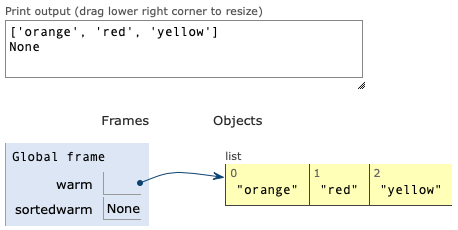
\includegraphics[width=\textwidth]{Figures/warm.png}
\end{figure}
\end{minipage}}%
\hfill
\adjustbox{valign=t}{\begin{minipage}[t]{0.49\textwidth}
\begin{table}[]
\begin{flushleft}
\begin{tabular}{ll}
\texttt{cool = ['grey', 'blue', 'green']} &  \\
\texttt{sortedcool = sorted(cool)} &  \\
\texttt{print(cool)} &  \\
\texttt{print(sortedcool)} &  \\
\end{tabular}
\end{flushleft}
\end{table}
\begin{figure}
	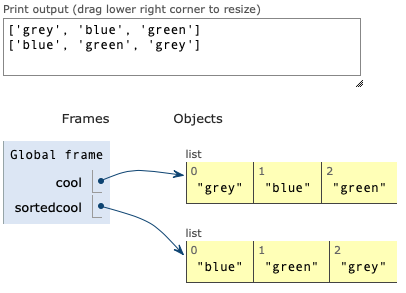
\includegraphics[width=0.9\textwidth]{Figures/cool.png}
\end{figure}
\end{minipage}}
\vfill
\end{frame}
%
\section{Aliasing \& Cloning}
\begin{frame}{Aliasing \& Cloning}
\vfill
\textbf{Aliasing}: if \texttt{a} refers to an object and you assign \texttt{b = a}, then both variables refer to the same object.\\
\vfill
\adjustbox{valign=t}{\begin{minipage}[t]{0.49\textwidth}
\begin{table}[]
\begin{flushleft}
\begin{tabular}{ll}
\texttt{>{}>{}> a = [1, 2, 3]} &  \\
\texttt{>{}>{}> b = a} &  \\
\texttt{>{}>{}> b is a} &  \\
\texttt{True} &  \\
\end{tabular}
\end{flushleft}
\end{table}
\end{minipage}}%
\hfill
\adjustbox{valign=t}{\begin{minipage}[t]{0.49\textwidth}
\begin{figure}
	
\includegraphics[width=0.5\textwidth]{Figures/aliasing.png}
\end{figure}
\end{minipage}}
\vfill
\begin{description}
	\item[Reference:] association of a variable with an object (in the example above, two references to the same object)
	\item[Aliased:] an object with more than one reference has more than one name, so we say that the object is \textit{aliased}.
\end{description}
\vfill
\end{frame}
%
\begin{frame}
\vfill
If the aliased object is mutable (like lists), changes made to one alias affect the other:
\vfill
\begin{table}[]
\begin{flushleft}
\begin{tabular}{ll}
\texttt{>{}>{}> a = [1, 2, 3]} &  \\
\texttt{>{}>{}> b = a} &  \\
\texttt{>{}>{}> b[0] = 42} &  \\
\texttt{>{}>{}> print(b)} &  \\
\texttt{[42, 2, 3]} &  \\
\texttt{>{}>{}> print(a)} &  \\
\texttt{[42, 2, 3]} &  \\
\end{tabular}
\end{flushleft}
\end{table}
\vfill
\begin{block}{Warning}
This aspect can be useful, but \textcolor{red}{error-prone}!
\end{block}
\begin{block}{Hint}
To be safe, \textcolor{red}{avoid aliasing} when working \textcolor{red}{with mutable objects}.
\end{block}
\vfill
\end{frame}
%
\begin{frame}
\vfill
The aliasing side-effect also holds for list methods we saw earlier:
\begin{table}[]
\begin{flushleft}
\begin{tabular}{ll}
\texttt{>{}>{}> warm = ['red', 'yellow', 'orange']} &  \\
\texttt{>{}>{}> hot = warm} &  \# we have an alias here\\
\texttt{>{}>{}> hot.append('pink')} &  \\
\texttt{>{}>{}> print(hot)} &  \\
\texttt{>{}>{}> print(warm)} &  \# Breakpoint 1\\
\texttt{>{}>{}> warm.sort()} &  \\
\texttt{>{}>{}> print(hot)} &  \\
\texttt{>{}>{}> print(warm)} &  \# Breakpoint 2\\
\end{tabular}
\end{flushleft}
\end{table}
\begin{figure}
     \centering
     \begin{subfigure}[b]{0.45\textwidth}
         \centering
         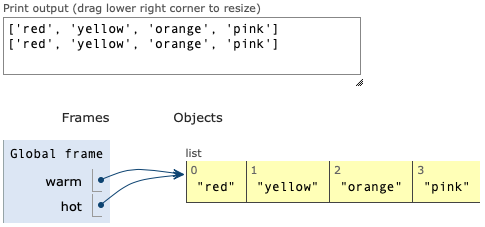
\includegraphics[width=\textwidth]{Figures/snap1}
         \caption{Breakpoint 1}
     \end{subfigure}
     \hfill
     \begin{subfigure}[b]{0.45\textwidth}
         \centering
         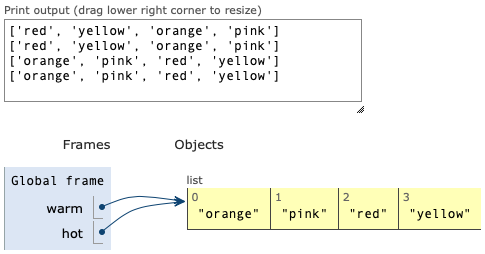
\includegraphics[width=\textwidth]{Figures/snap2}
         \caption{Breakpoint 2}
     \end{subfigure}
\end{figure}
\vfill
\end{frame}
%
\begin{frame}
\vfill
\textbf{Cloning}: create a new list (different object) by copying every element via assignment \texttt{b = a[:]}
\begin{table}[]
\begin{flushleft}
\begin{tabular}{ll}
\texttt{>{}>{}> cool = ['blue', 'green', 'grey']} &  \\
\texttt{>{}>{}> chill = cool[:]} &  \# we have a clone here\\
\texttt{>{}>{}> chill.append('black')} &  \\
\texttt{>{}>{}> print(cool)} &  \\
\texttt{>{}>{}> print(chill)} &  \\
\end{tabular}
\end{flushleft}
\end{table}
%\vfill
\begin{figure}
\centering
	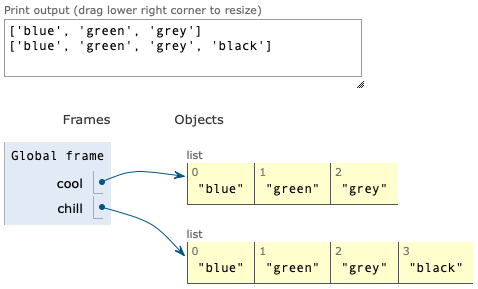
\includegraphics[width=0.5\textwidth]{Figures/clone.png}
\end{figure}
\vfill
\end{frame}
%
\begin{frame}
\vfill
\begin{block}{Warning}
Never mutate a list as you iterate through it.
\end{block}
Example: write a function that removes duplicates from two lists.
\vfill
\adjustbox{valign=t}{\begin{minipage}[t]{0.49\textwidth}
\begin{table}[]
\begin{flushleft}
\begin{tabular}{ll}
\texttt{def remove\_dups(L1, L2):} &  \\
\texttt{\quad for item in L1:} &  \\
\texttt{\quad\quad if item in L2:} &  \\
\texttt{\quad\quad\quad L1.remove(item)} &  \\
\texttt{\quad return L1} &  \\
\end{tabular}
\end{flushleft}
\end{table}
\end{minipage}}%
\hfill
\adjustbox{valign=t}{\begin{minipage}[t]{0.49\textwidth}
\begin{table}[]
\begin{flushleft}
\begin{tabular}{ll}
\texttt{def remove\_dups(L1, L2):} &  \\
\texttt{\quad L1copy = L1[:]} &  \\
\texttt{\quad for item in L1copy:} &  \\
\texttt{\quad\quad if item in L2:} &  \\
\texttt{\quad\quad\quad L1.remove(item)} &  \\
\texttt{\quad return L1} &  \\
\end{tabular}
\end{flushleft}
\end{table}
\end{minipage}}
\vspace{-0.4cm}
\vfill
\begin{table}[]
\begin{flushleft}
\begin{tabular}{ll}
\texttt{L1 = [1,2,3,4]} &  \\
\texttt{L2 = [1,2,5,6]} &  \\
\texttt{print(remove\_dups(L1, L2))} & \# left panel returns \texttt{[2, 3, 4]} \\
\texttt{print(remove\_dups(L1, L2))} & \# right panel returns \texttt{[3, 4]} \\
\end{tabular}
\end{flushleft}
\end{table}
\vfill
Left panel is incorrect. Why?
\begin{itemize}
	\item Python uses an internal counter to keep track of the position in the loop
	\item Mutation changes the length, but Python does not update the counter
	\item The loop never visits element \texttt{2} in \texttt{L1}
\end{itemize}
\vfill
\end{frame}
%
\section{Nesting}
\begin{frame}{Nesting}
\begin{block}{Recall}
Lists can be heterogeneous. An element of a list can itself be a list.
\end{block}
\begin{block}{Warning}
Mutation and aliasing affect also nested lists.
\end{block}
%\begin{table}[]
%\begin{flushleft}
%\begin{tabular}{ll}
%\texttt{warm = ['yellow', 'orange']} &  \\
%\texttt{hot = ['red']} &  \\
%\texttt{brightcolors = [warm]} \\
%\texttt{brightcolors.append(hot)} \\
%\texttt{print(brightcolors)} \\
%\texttt{hot.append('pink')} \\
%\texttt{print(hot)} \\
%\texttt{print(brightcolors)} \\
%\end{tabular}
%\end{flushleft}
%\end{table}
%
\adjustbox{valign=t}{\begin{minipage}[t]{0.49\textwidth}
\begin{table}[]
\begin{flushleft}
\begin{tabular}{ll}
\texttt{warm = ['yellow', 'orange']} &  \\
\texttt{hot = ['red']} &  \\
\texttt{brightcolors = [warm]} \\
\texttt{brightcolors.append(hot)} \\
\texttt{print(brightcolors)} \\
\texttt{hot.append('pink')} \\
\texttt{print(hot)} \\
\texttt{print(brightcolors)} \\
\end{tabular}
\end{flushleft}
\end{table}
\end{minipage}}%
\hfill
\adjustbox{valign=t}{\begin{minipage}[t]{0.49\textwidth}
\begin{figure}
	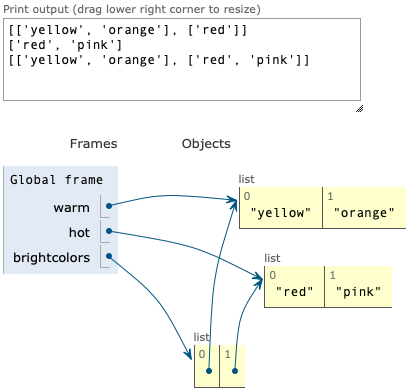
\includegraphics[width=0.75\textwidth]{Figures/nested.png}
\end{figure}
\end{minipage}}
\end{frame}
%------------------------------------------------------------------------------
%\section{References}
%\begin{frame}[allowframebreaks]{References}
%%\bibliographystyle{apacite}
%\printbibliography[heading=none]
%\end{frame}
\section{References}
\begin{frame}{References}
\begin{itemize}
	\item Guttag, J. V. (2013). \textit{Introduction to Computation and Programming using Python (Revised and Expanded Edition)}. MIT Press. [Sections 5.2 and 5.4]
	\item Downey, A. (2015). \textit{Think Python}. Green Tea Press ed. 2nd. [Chapter 10]
\end{itemize}
\end{frame}
%------------------------------------------------------------------------------
\section{Acknowledgments}
\begin{frame}{Acknowledgments}
% \begin{itemize}
% 	\item Prof. Irene Finocchi (LUISS University)\\
% 	\quad \textit{Introduction to Computer Programming} Lecture Notes (2020-2021)
% \end{itemize}
\end{frame}
%------------------------------------------------------------------------------
%\subsection{Sites legais}
%\begin{frame}{Sites legais}
%  Want to know more? See!
%  \begin{itemize}
%    \item Browse in my page \url{http://www.ezefranca.com}.
%    \item Browse on BCC page \url{http://www.sp.senac.br/bcc}.
%    \item Thanks WriteLaTeX from Support! \url{http://www.writelatex.com}.
%  \end{itemize}
%
%\end{frame}
%------------------------------------------------------------------------------

% -----------------------------------------------------------------------------
\end{document}
%-----------------------------------------------Este comentario nunca aparecera
